\documentclass{article}
\usepackage{amsmath}
\usepackage{amssymb}
\usepackage[pdftex]{graphicx}
\usepackage[framed,numbered,autolinebreaks,useliterate]{mcode}
\lstset{breakatwhitespace=false}

\pdfpagewidth 8.5in
\pdfpageheight 11in
\topmargin -1in
\headheight 0in
\headsep 0in
\textheight 8.5in
\textwidth 6.5in
\oddsidemargin 0in
\evensidemargin 0in
\headheight 50pt
\headsep 0in
\footskip .75in

\title{STA 601 - Homework 11}
\author{Kedar Prabhudesai}
\date{October 23, 2013}

\begin{document}
\maketitle

\noindent {\Large\underline{\textbf{Bayesian Model Selection:}}}\\

\underline{\textbf{Data:}}\\
\begin{align*}
y^n \sim Binomial(n,\theta).
\end{align*}

\underline{\textbf{Hypotheses:}}\\
\begin{align*}
H_0: \theta = 0.5\\
H_1: \theta \neq 0.5.
\end{align*}

\underline{\textbf{Prior on Hypotheses/Models:}}\\
\begin{align*}
p(H_0) = 0.5\\
p(H_1) = 0.5.
\end{align*}

\underline{\textbf{Prior on Parameter of the model:}} Let's use a Uniform prior, $\alpha = \beta = 1.$\\
\begin{align*}
\theta \sim Beta(\alpha,\beta).\\
\end{align*}

\underline{\textbf{Likelihood under each hypotheses:}} $k$ denotes number of heads.\\
\begin{align*}
L(y^n \mid H_0) &= \binom{n}{k}0.5^{k}0.5^{(n-k)} = \binom{n}{k}0.5^{n}.\\
L(y^n \mid H_1) &= \int_0^1{\binom{n}{k}\theta^{k}(1-\theta)^{(n-k)}\pi(\theta)}d\theta\\
&= \int_0^1{\binom{n}{k}\theta^{k}(1-\theta)^{(n-k)}}\times \frac{\theta^{\alpha-1}(1-\theta)^{\beta-1}}{B(\alpha,\beta)}d\theta\\
&= \frac{\binom{n}{k}}{B(\alpha,\beta)}\int_0^1{\theta^{\alpha+k-1}(1-\theta)^{(n+\beta-k-1)}}d\theta\\
&= \frac{\binom{n}{k}}{B(\alpha,\beta)}\times B(\alpha+k,n+\beta-k)\int_0^1{\frac{\theta^{\alpha+k-1}(1-\theta)^{(n+\beta-k-1)}}{B(\alpha+k,n+\beta-k)}}d\theta\\
\therefore L(y^n \mid H_1) &= \frac{\binom{n}{k}B(\alpha+k,n+\beta-k)}{B(\alpha,\beta)}
\end{align*}

\underline{\textbf{Posteriors:}}\\

Assuming, $p(H_0) = p(H_1) = 0.5.$\\
\begin{align*}
P(H_1 \mid y^n) &= \frac{L(y^n \mid H_1) p(H_1)}{L(y^n)}\\
&= \frac{L(y^n \mid H_1) p(H_1)}{L(y^n \mid H_0)p(H_0) + L(y^n \mid H_1)p(H_1)}\\
&= \frac{L(y^n \mid H_1)}{L(y^n \mid H_0) + L(y^n \mid H_1)}\\
P(H_1 \mid y^n) &= \frac{1}{1 + \frac{L(y^n \mid H_0)}{L(y^n \mid H_1)}}
\end{align*}

$\frac{L(y^n \mid H_0)}{L(y^n \mid H_1)}$ is Bayes' Factor in favor of $H_0.$\\
\begin{align*}
\therefore \frac{L(y^n \mid H_0)}{L(y^n \mid H_1)} = \frac{0.5^{n} B(\alpha,\beta)}{B(\alpha+k,n+\beta-k)}
\end{align*}

Similarly we can prove,
\begin{align*}
P(H_0 \mid y^n) &= \frac{1}{1 + \frac{L(y^n \mid H_1)}{L(y^n \mid H_0)}}
\end{align*}

$\frac{L(y^n \mid H_1)}{L(y^n \mid H_0)}$ is Bayes' Factor in favor of $H_1.$\\
\begin{align*}
\therefore \kappa = \frac{L(y^n \mid H_1)}{L(y^n \mid H_0)} = \frac{B(\alpha+k,n+\beta-k)}{0.5^{n}B(\alpha,\beta)}
\end{align*}

Based on value of $\kappa$ we can choose an appropriate model. If $\kappa > 1$, we are more in favor of $H_1,$ whereas if $\kappa < 1$, we are more in favor of $H_0.$\\

\pagebreak

\underline{\textbf{Asymptotic Behavior:}}\\

\indent If $n = 1,$ $\kappa = \frac{L(y^n \mid H_1)}{L(y^n \mid H_0)} = \frac{B(\alpha+k,1+\beta-k)}{0.5 B(\alpha,\beta)}.$ Hence, $\kappa$ will depend on the parameters of our prior, and the outcome $k$ that we get for the one coin flip. Using, $\alpha = \beta = 1,$ we always get $\kappa = 1,$ no matter what the outcome of the flip is! However, using different values of $\alpha,\beta$ will change what model we select based on the outcome of the flip.\\

\indent As $n \rightarrow \infty,$ we have $0.5^n \rightarrow 0,$ as a result of which $\kappa \rightarrow \infty,$ and does not depend on the outcomes of flips. This means that we always accept $H_1.$ The prior parameters $\alpha,\beta$ will only determine at what asymptotic value $\kappa$ comes very large. This is demonstrated in the following figures.\\

\begin{left}
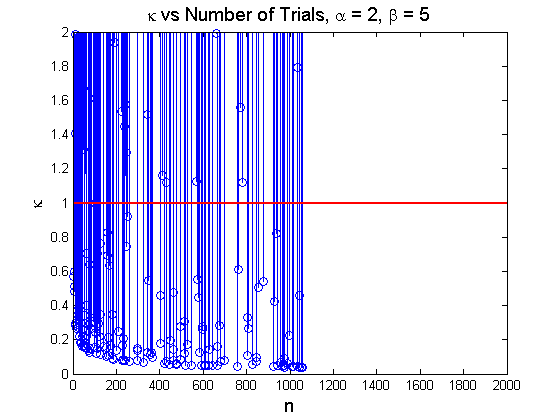
\includegraphics[scale=0.5]{KvsA2B5.png}
\end{left}
\begin{right}
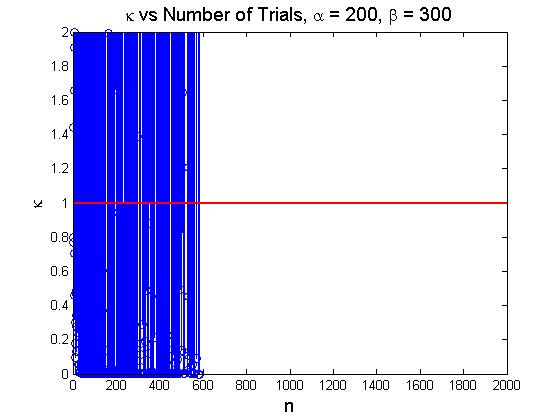
\includegraphics[scale=0.5]{KvsA200B300.png}\\
\end{right}

\underline{\textbf{Simulate Data:}}\\ 

Assume, under $H_0,$ $\theta = 0.5,$ and $H_1,$ $\theta \neq 0.5.$ To simulate $H_1,$ we draw $\theta$ randomly between $[0,1].$ We get the expected behavior, we are always in favor of $H_1$ after  around 1100 trials. This is confirmed by plotting both $\kappa$ and $1/\kappa.$\\

\begin{left}
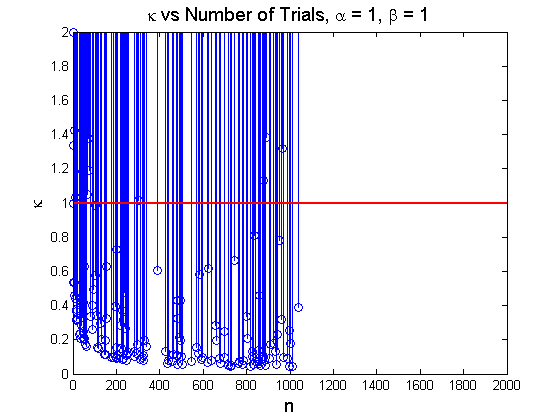
\includegraphics[scale=0.5]{KA1B1.png}
\end{left}
\begin{right}
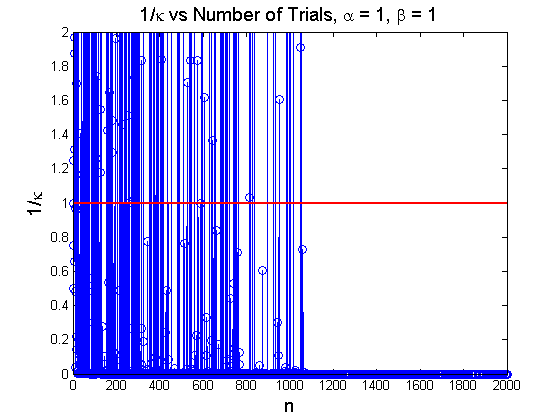
\includegraphics[scale=0.5]{1overKA1B1.png}\\
\end{right}

\pagebreak
\noindent {\Large\underline{\textbf{Appendix:}}}\\
\lstinputlisting{C:/Users/ksp6/Documents/Classes/2013-Fall/STA601-BayesAndModStats/homeworks/hw11/hw11.m}

\end{document}